\chapter{Studi Literatur}

\section{\textit{Reinforcement Learning} dan \textit{Q-Learning}}
\subsection{\textit{Reinforcement Learning}}

\textit{Reinforcement learning} (RL) merupakan sebuah kerangka pembelajaran sebuah kerangka pengembangan sebuah agen otonom yang dapat membuat suatu keputusan dalam ruang lingkup permasalahan yang terbatas. Secara umum, berikut merupakan formulasi sederhana dari kerangka \ac{RL}.

\begin{equation}
	\pi(s,a)^* = argmax(V(s,a))
\end{equation}

\(\pi\) merupakan notasi dari hasil fungsi kebijakan (\textit{policy}) yang merupakan keluaran dari \ac{RL}. Terdapat dua input untuk fungsi kebijakan tersebut, yaitu state (\(s\)) dan aksi (\(\alpha\)). Hasil yang diinginkan dari fungsi tersebut, adalah didapatkannya aksi yang terbaik dengan hasil evaluasi sebuah fungsi penilai (\(V\)). Berikut merupakan contoh dari penggunaan \ac{RL} pada Gambar \ref{fig:ilustrasi-RL} sebagai ilustrasi cara kerja fungsi kebijakan.

\begin{figure}[h]
	\centering
	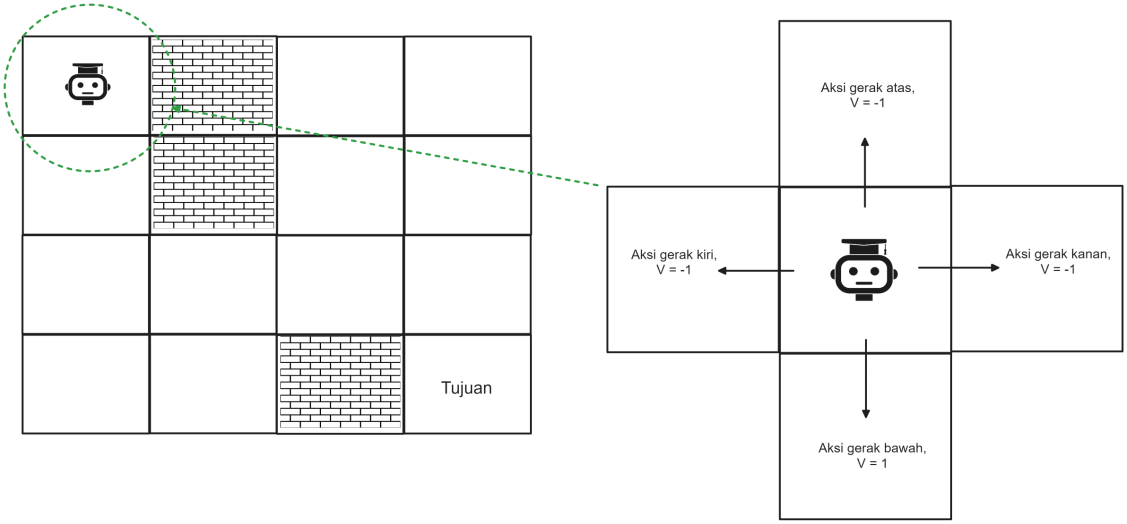
\includegraphics[width=0.8\textwidth]{chapter-2/ilustrasi-RL.png}
	\caption{Ilustrasi \ac{RL}}
	\label{fig:ilustrasi-RL}
\end{figure}


Pada Gambar \ref{fig:ilustrasi-RL}, tergambarkan sebuah ilustrasi agen otonom yang berada pada sebuah konfigurasi labirin. Pada setiap posisi (\textit{state}), terdapat empat aksi yang dapat diambil oleh agen otonom tersebut: gerak kanan, gerak kiri, gerak atas, dan gerak bawah. Masing-masing aksi akan memiliki sebuah nilai yang diberikan oleh fungsi \(V\). Pada contoh Gambar \ref{fig:ilustrasi-RL}, nilai fungsi \(V\) ketika agen berjalan menuju tempat kosong akan bernilai 1 dan akan bernilai -1 untuk sebaliknya. Fungsi kebijakan pada \ac{RL}, akan meninjau nilai hasil fungsi \(V\) berdasarkan masukan seluruh aksi pada posisi tersebut dan akan memilih aksi yang menghasilkan nilai fungsi \(V\) terbesar. Pada kasus diatas, Gambar \ref{fig:ilustrasi-RL}, aksi yang akan diambil adalah aksi gerak bawah. Berdasarkan ilustrasi tersebut, dapat diperhatikan bahwa fungsi \(V\) merupakan

Pada kasus diatas, Gambar 2.1, aksi yang akan diambil adalah aksi gerak bawah. Berdasarkan ilustrasi tersebut, dapat diperhatikan bahwa fungsi \(V\) merupakan esensi dari pengembangan agen \ac{RL} yang mumpuni. Fungsi \(V\) yang optimal, akan menghasilkan agen \ac{RL} yang optimal. Konstruksi fungsi \(V\) dapat dilakukan dengan berbagai metode. Pada sistem yang sederhana, fungsi \(V\) bahkan dapat diatur secara manual oleh pengembang sistem. Namun, agar fungsi \(V\) tersebut dapat berubah secara dinamik, mengikuti konfigurasi state yang mungkin berubah, agen \ac{RL} dapat dilatih menggunakan metode \textit{Q-Learning}.

\subsection{\textit{Q-Learning}}
\textit{Q-Learning} merupakan sebuah metode yang dapat digunakan untuk melakukan konstruksi fungsi penilai yang optimal untuk membangun fungsi kebijakan pada \ac{RL}. \textit{Q-Learning} menggunakan algoritma yang marak digunakan pada pengembangan agen \ac{RL} karena merupakan algoritma yang memiliki konvergensi yang stabil \parencite{lim2022regularized}. Cara kerja \textit{Q-Learning} dapat dirangkum menggunakan persamaan berikut.

\begin{equation}
	\label{eq:q-learning}
	Q_{new}(s_t,a_t) = (1-\alpha) Q(s_t, a_t) + \alpha (r_t + \gamma \cdot maxQ(s_{t+1},a))
\end{equation}

\(Q\) merupakan alternatif bentuk fungsi \(V\) yang memiliki dimensi terbatas, sebesar banyaknya aksi \(\times\) banyaknya \textit{state}. \(Q\) sering dilihat sebagai sebuah \textit{lookup table}, disebut \textit{Q-Table}, yang memiliki nilai diskrit untuk posibilitas keluaran nilai aksi berdasarkan \textit{state} terkini. Berikut, pada Gambar \ref{fig:ilustrasi-qtable}, merupakan ilustrasi dari \textit{Q-Table}.

\begin{figure}[h]
	\centering
	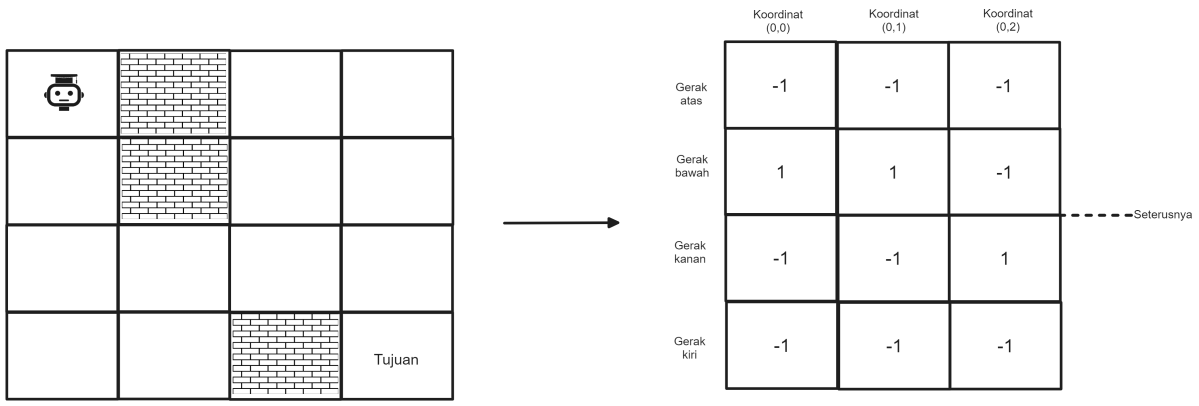
\includegraphics[width=1\textwidth]{chapter-2/ilustrasi-qtable.png}
	\caption{Ilustrasi \textit{Q-Table}}
	\label{fig:ilustrasi-qtable}
\end{figure}

Pada ilustrasi Gambar \ref{fig:ilustrasi-qtable}, \textit{Q-Table} merupakan representasi hasil translasi seluruh \textit{state} (dalam bentuk koordinat) beserta seluruh aksi yang menghasilkan sebuah tabel pencarian yang dapat menghasilkan keluaran fungsi penilai dengan hanya index dari tabel tersebut menggunakan \textit{state} dan aksi.

Dengan representasi tersebut, Persamaan 2.2 dapat dipahami sebagai pembaruan nilai \textit{Q-Table} pada index (\(s\), \(a\)) dengan beberapa proporsi nilai \textit{Q-Table} sebelumnya, ditambah dengan penjumlahan dari keluaran fungsi penilai saat itu dan fungsi penilai setelah pengambilan fungsi tersebut. Berikut merupakan detail dari penjelasan tersebut.


\begin{enumerate}
	\item \((1-\alpha) Q(s_t,a_t)\): merupakan nilai \textit{Q-Table} yang akan diupdate, namun informasinya masih digunakan untuk mendapatkan nilai yang optimal sesuai dengan prinsip \textit{Markov Decision Process}.
	\item \(\alpha (r_t + \gamma \cdot maxQ(s_{t+1},a))\): merupakan nilai pembaruan \textit{Q-table} yang berasal dari keluaran fungsi penilai aksi pada state sekarang (\(r_t\)) dan sedikit kontribusi (bergantung \(\gamma\)) dari prediksi fungsi penilai pada state selanjutnya \(maxQ(s_{t+1},a)\).
\end{enumerate}



\section{\acl{RL} dalam Sistem Kontrol}

\ac{RL}, sebagai kerangka agen otonom, merupakan salah satu alternatif yang bagus sebagai sistem komplementer maupun utama dari sebuah sistem kontrol. Hal tersebut merupakan akibat dari kapabilitas \ac{RL} untuk menentukan sinyal kontrol. yang dekat ke nilai optimal dengan cara \textit{trial-and-error} \parencite{vichugov2005application}. Secara umum, sistem RL yang dikembangkan dapat menjadi tambahan \textit{feedback loop} dari sebuah sistem kontrol diskrit yang dapat diilustrasikan pada Gambar \ref{fig:RL-loop-kontrol}.


\begin{figure}[H]
	\centering
	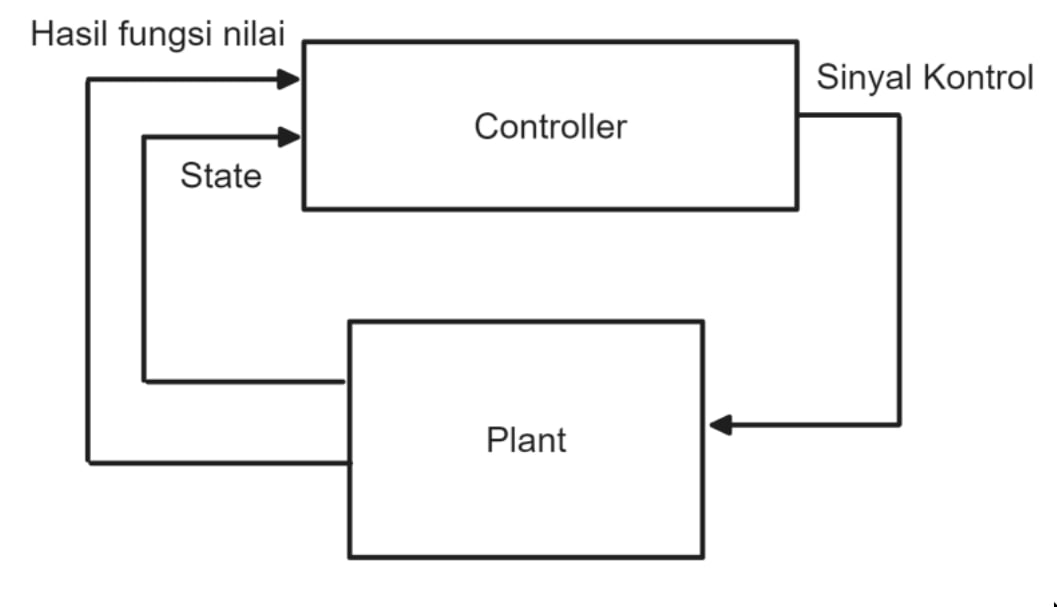
\includegraphics[width=0.8\textwidth]{chapter-2/RL-kontrol-loop.jpg}
	\caption{Diagram Feedback Loop \ac{RL} pada Sistem Kontrol \parencite{vichugov2005application}}
	\label{fig:RL-loop-kontrol}
\end{figure}

Pada Gambar \ref{fig:RL-loop-kontrol}, digambarkan sebuah kerangka \ac{RL} yang menggunakan keluaran sinyal kontrol sebagai aksi, keluaran \textit{plant} sebagai \textit{state}, dengan fungsi nilai yang diformulasikan bersesuaian dengan fisis yang ada pada \textit{plant}. Permasalahan \textit{cart pole balancing} \parencite{nagendra2017comparison} merupakan salah satu contoh sistem kontrol klasik yang marak digunakan untuk \textit{benchmarking} performa agen \ac{RL}. Berikut, pada Gambar \ref{fig:cartpole-illustration}, merupakan ilustrasi dari permasalahan \textit{cart pole balancing}.

\begin{figure}[h]
	\centering
	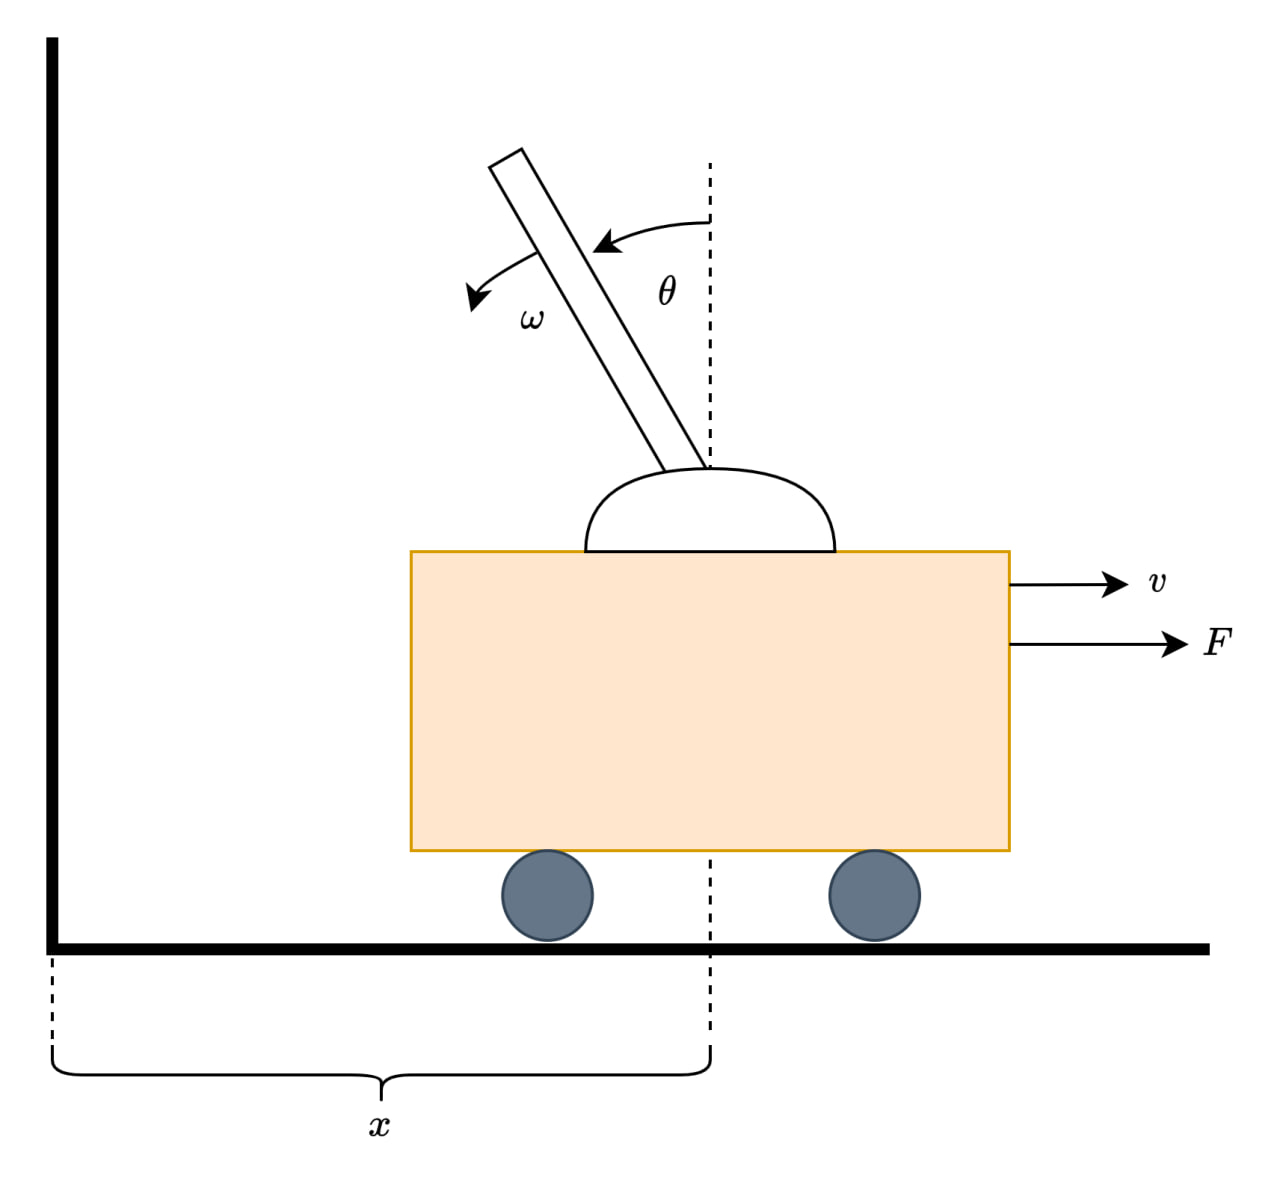
\includegraphics[width=0.6\textwidth]{chapter-2/cartpole-illustration.jpg}
	\caption{Ilustrasi Permasalahan \textit{Cart Pole Balancing}}
	\label{fig:cartpole-illustration}
\end{figure}

Pada sistem fisis sederhana Gambar \ref{fig:cartpole-illustration}, didefinisikan masing-masing variabel dari kerangka \ac{RL} sebagai berikut.

\begin{enumerate}
	\item \textit{State}: \(\theta\), \(\omega\), \(v\), dan \(x\)
	\item Aksi: \(F\)
\end{enumerate}

Kasus permasalahan \textit{Cart Pole Balancing}, sebagaimana kasus kontrol klasik lainnya, memerlukan sistem komputasi yang memiliki \textit{time delay} (\(t_d\)) yang kecil bila diimplementasikan pada sistem nyata. Bila \(t_d\) terlalu besar, maka sistem dapat menjadi tidak stabil sehingga tidak berhasil dikontrol oleh perhitungan dari agen \ac{RL}.

Seiring dengan semakin maraknya perkembangan \ac{RL}, sudah banyak kasus yang mengadopsi kerangka ini untuk digunakan pada sistem kontrol yang lebih kompleks [1, 2, 3]. Sehingga, \ac{RL} dapat tetap digunakan tanpa mengakibatkan ketidakstabilan pada sistem kontrol, maka diperlukan mekanisme universal yang dapat digunakan untuk mempercepat iterasi perhitungan RL pada \textit{processor} komputer.


\section{\acl{FPGA}}
\label{sec:fpga}

\acf{FPGA} merupakan sebuah perangkat keras yang mampu direkonfigurasi menggunakan sebuah bahasa \ac{HDL} \parencite{smith2024FPGA}. \ac{FPGA}, sebagai perangkat keras yang \textit{reconfigurable}, mulai marak digunakan sebagai basis perangkat keras untuk mendesain maupun mengimplementasikan akselerator perangkat keras untuk optimasi permasalahan komputasi \parencite{gerlach2023fpgaplacement}.

Secara prinsip, \ac{FPGA} terdiri atas \textit{Configurable Logic Blocks} yang dibangun diatas rangkaian \textit{Look Up Table}. Ilustrasi internal dari \ac{FPGA} dapat ditinjau pada gambar \ref{fig:ilustrasi-internal-fpga}.

\begin{figure}[h]
	\centering
	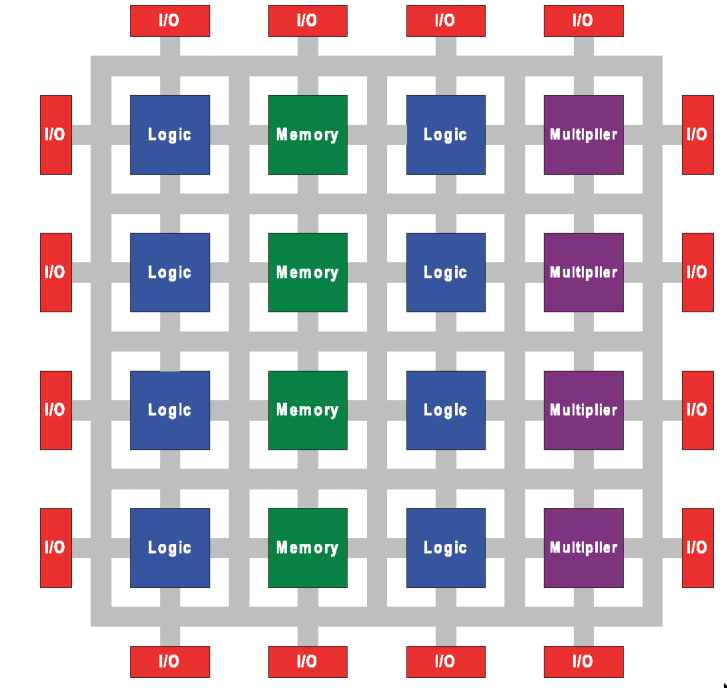
\includegraphics[width=0.6\textwidth]{chapter-2/fpga-internal.jpg}
	\caption{Ilustrasi internal \ac{FPGA} \parencite{md2015field}}
	\label{fig:ilustrasi-internal-fpga}
\end{figure}

Pada tugas akhir ini, akselerator perangkat keras yang akan diimplementasikan dan diuji pada \ac{FPGA}. Perangkat \ac{FPGA} yang digunakan adalah Nexys A7-100T yang memiliki spesifikasi sebagaimana dideskripsikan oleh tabel \ref{tab:nexys-specs}.

\begin{table}[h]
	\caption{Spesifikasi \ac{FPGA} Nexys A7-100T}
	\label{tab:nexys-specs}
	\vspace{0.25cm}
	\begin{center}
		\begin{tabular}{|c|c|}
			\hline
			Komponen Perangkat Keras        & Jumlah \tabularnewline
			\hline
			\textit{\ac{LUTs}}              & 63.400 \tabularnewline
			\textit{Flip-flops}             & 126.800 \tabularnewline
			\textit{Block \ac{RAM}}         & 4.860 Kb \tabularnewline
			\textit{DSP Slices}             & 240 \tabularnewline
			\textit{Clock Management Tiles} & 6 \tabularnewline
			\hline
		\end{tabular}
	\end{center}
\end{table}

Hasil desain akselerator, akan kemudian dilihat efisiensinya dengan mengacu kepada penggunaan jumlah penggunaan komponen perangkat keras yang tercantum pada tabel \ref{tab:nexys-specs}.


\section{Akselerator Perangkat Keras untuk \acl{RL}}
\label{sec:accelerator-researches}

Sebelum penelitian tugas akhir ini, terdapat beberapa pengembangan akselerator perangkat keras untuk \ac{RL} yang diimplementasikan pada \ac{FPGA}. Berdasarkan \parencite{sutisna2023faraneq}, pengembangan akselerator perangkat keras untuk \ac{RL} menggunakan teknik \textit{Q-Learning} itu pertama kali dikembangkan oleh Da Silva et al pada \parencite{dasilva2019parallel}. Implementasi yang dikembangkan pada \parencite{dasilva2019parallel} berfokus untuk mengoptimalisasi perhitungan pada persamaan \ref{eq:q-learning} menggunakan teknik perhitungan paralel yang diilustrasikan pada gambar \ref{fig:ilustrasi-dasilvi}.

\begin{figure}[h]
	\centering
	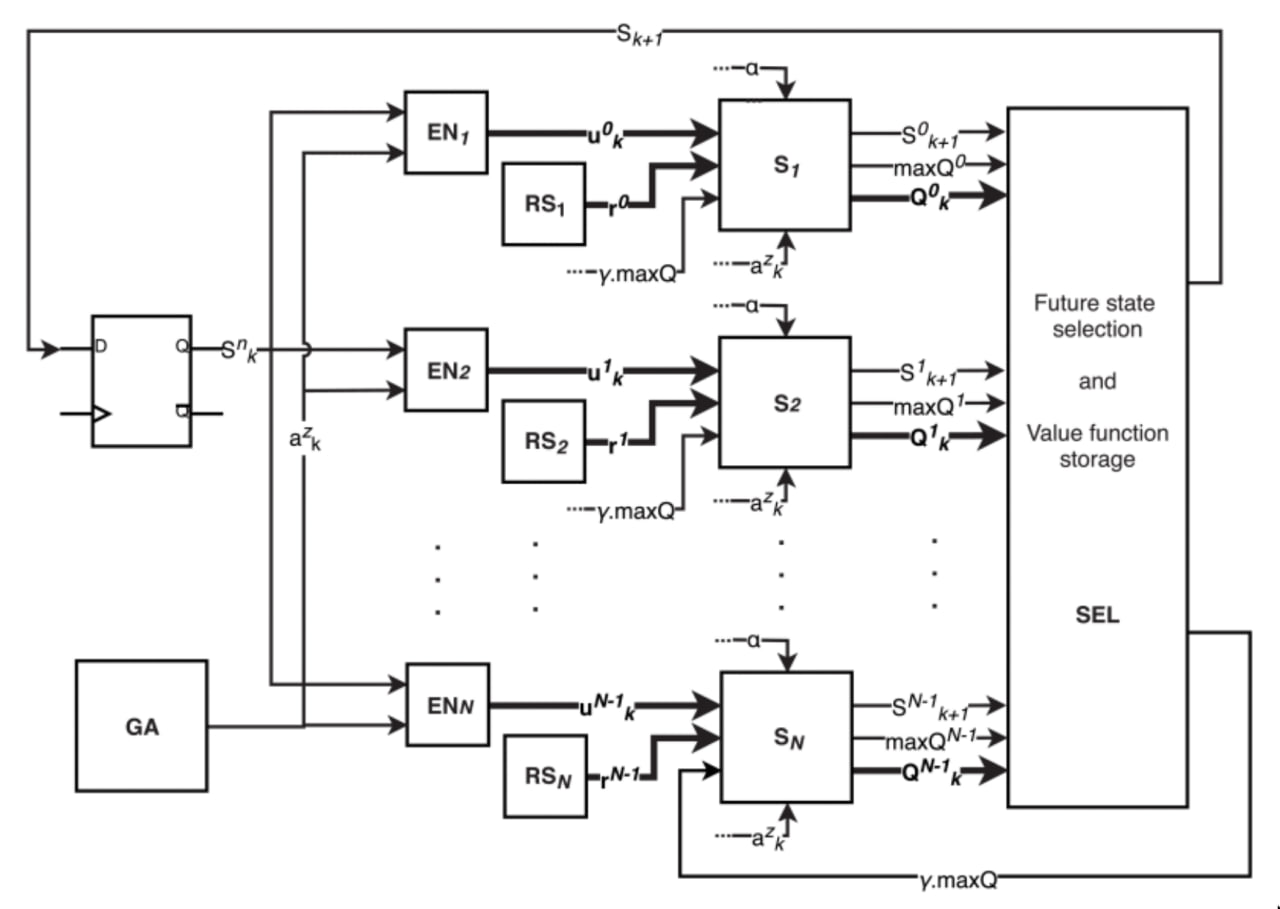
\includegraphics[width=0.8\textwidth]{chapter-2/dasilvi.jpg}
	\caption{Ilustrasi teknik perhitungan paralel \parencite{dasilva2019parallel}}
	\label{fig:ilustrasi-dasilvi}
\end{figure}

Teknik perhitungan paralel tersebut berhasil mendapat kecepatan \textit{throughput} sebesar 13.4  \ac{MSps} untuk \textit{Q-Table} yang memiliki 132 \textit{state} dan 4 aksi. Lalu, ada pula implementasi akselerator perangkat keras dari Spanò et al \parencite{spano2019efficient}. Arsitektur akselerator perangkat keras yang dikembangkan oleh \parencite{spano2019efficient} merupakan akselerator yang memanfaatkan penggunaan \textit{internal} \ac{RAM} \textit{block} untuk menyimpan \textit{Q-Table} dan melakukan perhitungan pada persamaan \ref{eq:q-learning} secara simultan. Gambar \ref{fig:ilustrasi-spano} menggambarkan arsitektur yang dirancang oleh \parencite{spano2019efficient}.

\begin{figure}[h]
	\centering
	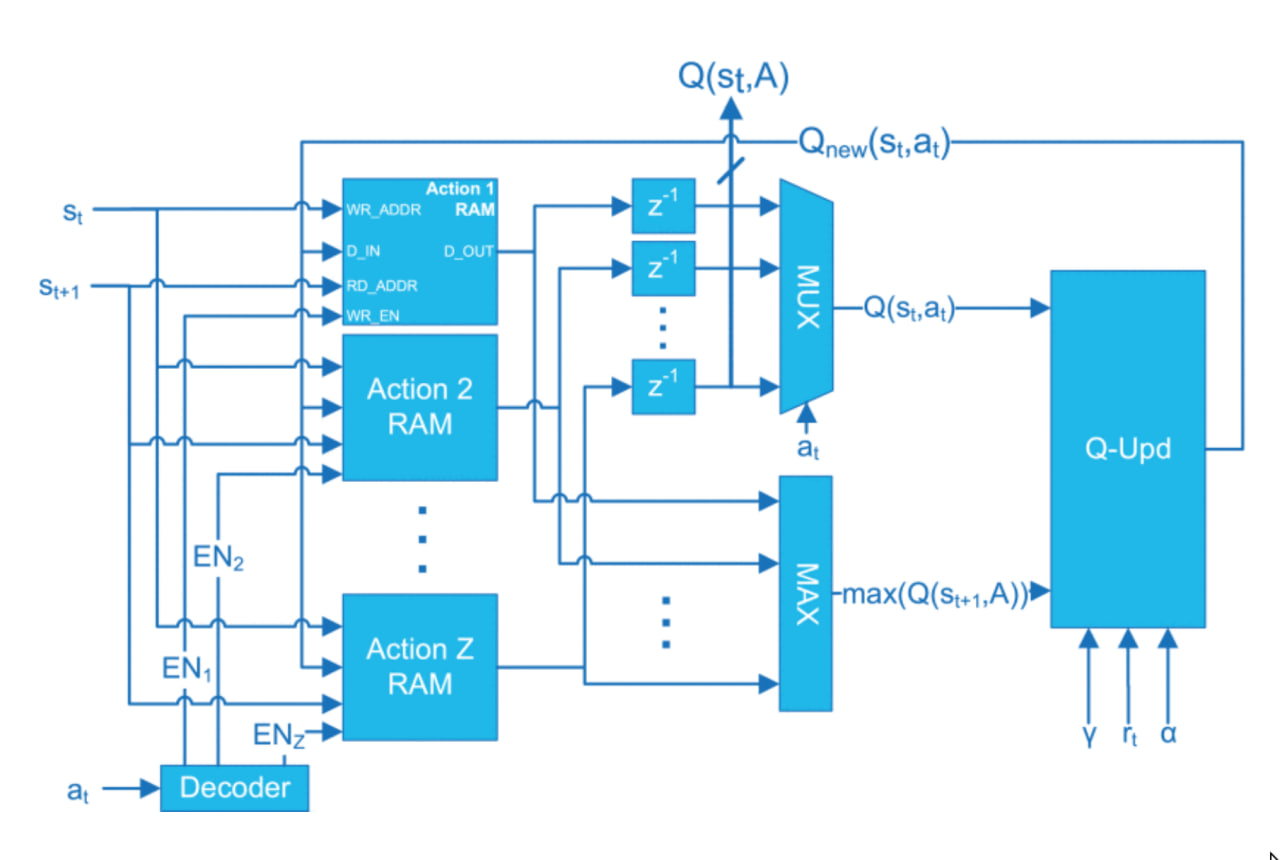
\includegraphics[width=0.8\textwidth]{chapter-2/spano.jpg}
	\caption{Ilustrasi arsitektur akselerator \parencite{spano2019efficient}}
	\label{fig:ilustrasi-spano}
\end{figure}

Akselerator perangkat keras dari \parencite{spano2019efficient} berhasil mendapatkan kecepatan \textit{throughput} sebesar 112 MSps untuk \textit{Q-Table} dengan 128 \textit{state} and 4 aksi. Arsitektur yang dikembangkan oleh \parencite{spano2019efficient}, merupakan akselerator \textit{Q-Learning} yang dapat digunakan secara \textit{Generic} karena implementasinya memberikan fleksibilitas kepada pengguna akselerator untuk membangun desain lingkungan agen \ac{RL}.

Pengembangan akselerator perangkat keras untuk \ac{RL} dengan performa paling tinggi, sejauh ini, merupakan desain yang dibuat oleh Sutisna et al \parencite{sutisna2023faraneq} yang menggunakan teknik paralelisme, \textit{pipelining}, dan berbagai implementasi teknik optimasi untuk perhitungan algoritma dari Persamaan \ref{eq:q-learning} seperti \textit{barrel shifter}  dan \textit{Fibonacci Linear Feedback Shift Register} \parencite{panda2012FPGA}. Arsitektur tersebut, diilustrasikan pada gambar \ref{fig:ilustrasi-faraneq}. Dengan teknik optimasi tersebut, akselerator pada \parencite{sutisna2023faraneq} berhasil mendapatkan kecepatan \textit{throughput} sampai dengan 148.55 MSps.

% Selain \parencite{spano2019efficient}, terdapat juga arsitektur akselerator \textit{Q-Learning Generic} lainnya yang didesain oleh Meng et al \parencite{meng2020generic}.

\begin{figure}[h]
	\centering
	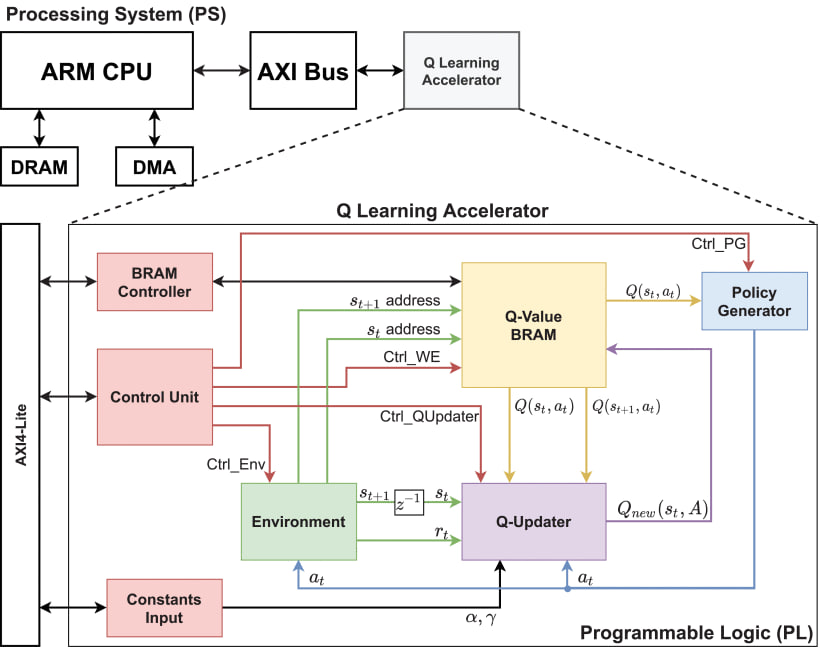
\includegraphics[width=0.8\textwidth]{chapter-2/faraneq.jpg}
	\caption{Ilustrasi arsitektur keseluruhan dari \parencite{sutisna2023faraneq}}
	\label{fig:ilustrasi-faraneq}
\end{figure}

Desain dari akselerator yang diajukan oleh \parencite{sutisna2023faraneq, dasilva2019parallel, panda2012FPGA} merupakan desain yang menggunakan prinsip separasi perangkat keras dan perangkat lunak menggunakan sistem \textit{Processing Systems-Processing Logic} (PS-PL) yang menghubungkan sebuah \textit{processor} sebagai PL dengan akselerator sebagai PS menggunakan sebuah bus dengan protokol tertentu, misalnya \textit{Advanced eXtensible Interface} (AXI) yang digunakan oleh \parencite{sutisna2023faraneq}.

Salah satu alternatif dari pendekatan desain PS-PL untuk mendesain akselerator adalah menggunakan ekstensi \ac{ISA}. \ac{ISA} adalah sebuah set instruksi yang ditentukan oleh sebuah arsitektur komputer yang menentukan perintah-perintah dasar yang dapat dilakukan oleh sebuah \textit{processor}. Riset yang dilakukan oleh Yang et al \parencite{yang2023design} adalah satu contoh penggunaan RISC-V untuk pengembangan akselerator perangkat keras. Akselerator pada \parencite{yang2023design} didesain untuk proses enkripsi pada perangkat \ac{IoT} dengan konsumsi daya rendah. Gambar \ref{fig:ilustrasi-lowiot} merupakan ilustrasi dari desain akselerator ekstensi \textit{processor} RISC-V pada \parencite{yang2023design}.

\begin{figure}[H]
	\centering
	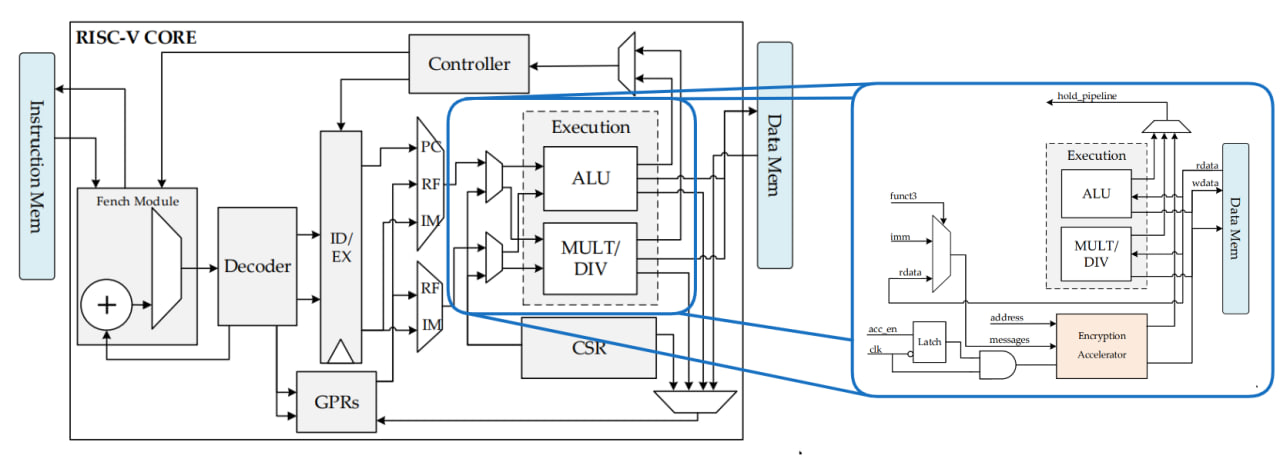
\includegraphics[width=1\textwidth]{chapter-2/lowiot.jpg}
	\caption{Arsitektur \textit{processor} RISC-V pada \parencite{yang2023design}}
	\label{fig:ilustrasi-lowiot}
\end{figure}

Kelebihan utama yang dimiliki oleh desain \parencite{yang2023design} adalah minimnya total penggunaan sumber daya perangkat keras dan minimnya \textit{delay} yang muncul dari transmisi data dari PS ke PL. Perancangan desain akselerator \ac{RL} yang menggunakan pendekatan sama dengan \parencite{yang2023design}, sampai penulisan tugas akhir ini, masih belum dilakukan. Sehingga, menjadi salah satu movitasi utama untuk melakukan eksplorasi desain akselerator \ac{RL} menggunakan \textit{processor} RISC-V.


\section{\textit{Processor} RISC-V VeeR EL2}
\label{sub:veer-el2}

RISC-V sebagai \ac{ISA} yang \textit{open}, memiliki banyak variasi \textit{processor} yang dikembangkan oleh berbagai perusahaan maupun individu lain. \textit{Processor} VeeR EL2 \parencite{chip2024cores} adalah satu \textit{processor} yang menggunakan RISC-V \ac{ISA}. VeeR EL2 merupakan \textit{processor} yang dikembangkan oleh Chip Alliance, ilustrasi arsitektur dari \textit{processor} secara ringkas dapat dilihat pada Gambar \ref{fig:veer-el2-short}.
% TODO: LAMPIRAN A

\begin{figure}[h]
	\centering
	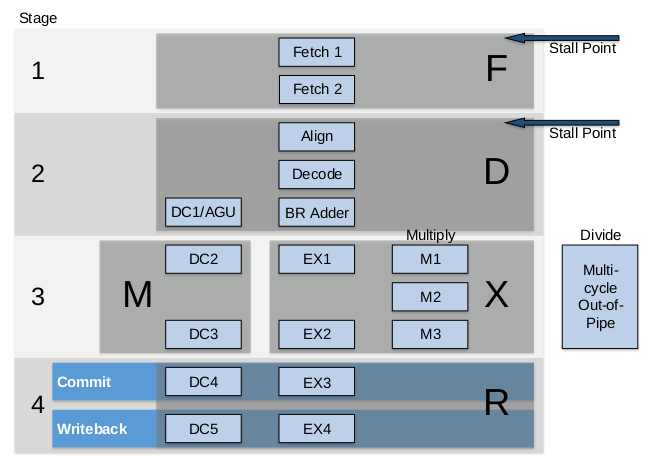
\includegraphics[width=0.8\textwidth]{chapter-2/veer-el2-short.png}
	\caption{Ilustrasi Singkat Arsiktektur VeeR EL2 \parencite{chip2024cores}}
	\label{fig:veer-el2-short}
\end{figure}

Deskripsi lebih detail, dari Gambar \ref{fig:veer-el2-short}, arsitektur VeeR EL2 dapat terdapat pada Lampiran A. Dari Gambar \ref{fig:veer-el2-short}, dapat diperhatikan bahwa VeeR EL2 merupakan \textit{processor} yang miliki lima \textit{pipeline stage} sebagai berikut.

\begin{enumerate}
	\setlength{\itemsep}{0pt}
	\setlength{\parskip}{0pt}
	\item \textit{Fetch}: \textit{Stage} ketika \textit{processor} mengambil instruksi dari memori.
	\item \textit{Decode}: \textit{Stage} ketika instruksi yang diambil diidentifikasi dan disesuaikan untuk operasi pada \textit{stage} \textit{execute} dan \textit{memory}.
	\item \textit{Execute} dan \textit{Memory}: \textit{Stage} yang melakukan operasi sesuai dengan diminta oleh \textit{stage decode}.
	\item \textit{Writeback}: \textit{Stage} yang menuliskan hasil dari instruksi yang dieksekusi kembali ke register atau memori jika diperlukan.
\end{enumerate}

VeeR EL2 memiliki kelebihan fleksibilitas dalam \textit{stage execute} dan \textit{memory} yang fleksibel untuk diimplementasikan sebuah ekstensi. Hal tersebut merupakan alasan dari pemilihan VeeR EL2 sebagai \textit{processor} yang dipilih untuk implementasi ekstensi \ac{ISA} RISC-V untuk akselerator \ac{RL} pada penelitian ini.


% \section{Kubernetes}

Kubernetes adalah \textit{platform open-source} yang digunakan untuk mengelola, otomatisasi, dan deployment aplikasi yang dikemas dalam container. Platform ini membantu mengelola infrastruktur aplikasi secara efisien dan konsisten. Kubernetes dirancang untuk dapat mengelola, secara otomatis, aplikasi yang berjalan pada lingkungan yang terdistribusi dan skala yang besar. Kubernetes berfokus pada konsep "\textit{container orchestration}", yang berarti kubernetes membantu mengatur dan mengelola container secara otomatis.

Kubernetes bekerja dengan mengolaborasikan komponen yang ada di dalamnya, diantaranya, \textit{node, pod, service,}dan \textit{deployment}. Secara umum, \textit{Node} adalah mesin fisik atau virtual dimana container dijalankan. \textit{Pod} merupakan unit terkecil dalam kubernetes dan berisi satu atau beberapa container yang berjalan bersamaan. \textit{Service} digunakan untuk mengakses aplikasi pada pod, sedangkan \textit{deployment} digunakan untuk melakukan konfigurasi pada \textit{pod} dan \textit{container}.

Kubernetes dilengkapi dengan fitur-fitur seperti \textit{auto scaling, load balancing,} dan \textit{self-recovery}, sehingga aplikasi pada kubernetes selalu tersedia dan terus berjalan bahkan akan mencoba untuk memperbaiki sendiri pada saat terjadi masalah atau kegagalan pada node atau aplikasi. Dengan fitur-fitur tersebut, kubernetes memudahkan dalam mengelola aplikasi yang kompleks pada lingkungan yang skala besar dan terdistribusi.
% 
% \subsection{Pod}
Pod adalah unit komputasi terkecil dalam lingkungan aplikasi yang dijalankan pada platform Kubernetes. Pod berisi lebih dari satu kontainer dan memiliki jaringan serta penyimpanan yang dipakai bersama serta spesifikasi untuk menjalankan kontainer didalamnya, \parencite{pod}.
Sebuah pod adalah abstraksi tingkat tinggi yang membungkus satu atau beberapa container. Sebuah pod pasti memiliki konfigurasi spesifikasi resource secara eksplisit. Pod bertanggung jawab untuk mengatur koneksi antara container yang berada dalam satu pod. Pod mungkin untuk memiliki sifat yang ephemeral, artinya dapat berubah-ubah dalam waktu singkat tergantung pada kebutuhan aplikasi, \parencite{ephemeral}. Hal ini memungkinkan aplikasi untuk beradaptasi dengan cepat terhadap perubahan kondisi lingkungan yang terjadi.
% 
% \subsection{\textit{Autoscaler}}
\textit{Autoscaler} adalah fitur pada Kubernetes yang memberikan akses ke pengguna untuk secara otomatis menyesuaikan jumlah replika atau utilisasi sumber daya dari sebuah \textit{deployment} atau \textit{replication controller} berdasarkan beban kerja aplikasi atau suatu metrik tertentu, contohnya jumlah \textit{request} per satuan waktu. \textit{Autoscaler} dapat diatur untuk menambahkan atau mengurangi jumlah replika atau batasan utilisasi sumber daya secara dinamis, sehingga dapat mengoptimalkan penggunaan sumber daya dan meningkatkan skalabilitas aplikasi.

\textit{Autoscaler} dapat disesuaikan dengan mengatur parameter tertentu, seperti target utilisasi CPU, beban kerja maksimum dan minimum, serta durasi pengecekan. Dengan pengaturan yang tepat, \textit{autoscaler} dapat membantu meningkatkan kinerja dan efisiensi aplikasi, serta memastikan aplikasi tetap berjalan normal bahkan ketika ada perubahan trafik atau gejolak jumlah \textit{request} ke suatu layanan.

Kubernetes menyediakan dua jenis \textit{autoscaler}, yaitu \textit{Horizontal Autoscaler} (HA) dan \textit{Vertical Autoscaler} (VA). HA bekerja dengan menambah atau mengurangi jumlah replika pod, sedangkan VA bekerja dengan menyesuaikan alokasi sumber daya pada pod yang sudah ada.
% 
% \subsubsection{\textit{Horizontal Autoscaler}}
\textit{Horizontal Autoscaler} (HA) adalah fitur pada Kubernetes yang melakukan penskalaan atau replikasi otomatis berdasarkan beban kerja atau metrik tertentu untuk menyesuaikan dengan kebutuhan, \parencite{hpa}. Dalam \textit{horizontal autoscaling}, jumlah \textit{instance} aplikasi dapat bertambah atau berkurang secara otomatis berdasarkan pengukuran metrik tertentu yang ditentukan oleh pengguna.

HA sendiri diatur oleh komponen Kubernetes yang disebut \textit{HorizontalPodAutoscaler} (HPA). Komponen HPA sendiri berfungsi agar pengguna dapat menentukan metrik yang digunakan untuk menentukan aksi replikasi. Metrik yang dipakai untuk menentukan dapat berupa CPU, memori, atau metrik kustom yang ditentukan oleh pengguna. Komponen HPA memberikan pengguna akses untuk memberikan batas atas dan batas bawah untuk jumlah \textit{instance} aplikasi, serta target penggunaan rata-rata untuk setiap \textit{instance}. Dengan konfigurasi yang tepat, HA dapat membantu meningkatkan ketersediaan aplikasi dan mengoptimalkan penggunaan sumber daya di lingkungan Kubernetes.
% 
% \subsubsection{\textit{Vertical Autoscaler}}
\textit{Vertical Autoscaler} (VA) merupakan mekanisme scaling pada Kubernetes yang menyesuaikan skala aplikasi dengan memanipulasi sumber daya CPU dan memori pada level kontainer atau pod.
Dibandingkan dengan HA, VA digunakan untuk otomatisasi pengaturan alokasi sumber daya aplikasi pada level yang lebih rendah dibandingkan dengan \textit{horizontal autoscaler} (jumlah replika pod).
VA berguna untuk mengotomasi reservasi CPU dan memori yang sesuai. 
Penyesuaian ini dapat meningkatkan kluster kubernetes spesifiknya pada utilitasi sumber daya karena dapat mengurangi alokasi CPU dan memori pada sebuah \textit{node} agar bisa dipakai oleh pod lain, \parencite{vpa2}.

Dalam sebuah thesis pascasarjana di KTH Royal Institute of Technology, Swedia, \parencite{predictiveva}, terdapat pembahasan penggunaan VA pada lingkungan Kubernetes dengan mengevaluasi dan membandingkan beberapa strategi VA, seperti \textit{resource-based} VA dan \textit{performance-based} VA. \textit{Resource-based} VA menentukan alokasi sumber daya berdasarkan penggunaan memori dan CPU, sedangkan \textit{performance-based} VA menentukan alokasi sumber daya berdasarkan performa aplikasi yang diukur dengan metrik tertentu. Hasil dari studi ini menunjukkan bahwa VA pada Kubernetes dapat membantu meningkatkan efisiensi penggunaan sumber daya dan performa aplikasi. Namun, pemilihan strategi VA yang tepat sangat bergantung pada kebutuhan dan karakteristik aplikasi yang akan di-\textit{deploy} pada Kubernetes.

% Selain itu, studi literatur yang dilakukan oleh Lu et al. pada tahun 2020 juga membahas tentang VA pada Kubernetes. Peneliti tersebut mengusulkan sebuah algoritma VA yang disebut sebagai Lightweight Vertical Autoscaler (LVA) yang menggunakan teknik regresi linier untuk memprediksi penggunaan sumber daya aplikasi pada level pod. Hasil pengujian menunjukkan bahwa LVA mampu mengalokasikan sumber daya secara efektif dan menghasilkan performa aplikasi yang lebih baik dibandingkan dengan strategi VA lainnya.

% Secara keseluruhan, studi literatur tersebut menunjukkan bahwa VA merupakan mekanisme scaling yang penting pada Kubernetes dan dapat membantu meningkatkan efisiensi penggunaan sumber daya dan performa aplikasi. Selain itu, ada beberapa strategi VA yang dapat dipilih, tergantung pada karakteristik dan kebutuhan aplikasi yang di-deploy pada Kubernetes.

% 
% \subsection{Kubernetes \textit{Client Library}}
Kubernetes \textit{Client Library} adalah sebuah perpustakaan atau \textit{Library} yang dapat digunakan oleh \textit{developer} atau \textit{administrator} untuk berinteraksi dengan Kubernetes API \parencite{clientlibrary}. Saat ini, Kubernetes sudah memiliki \textit{library} resmi pada bahasa pemrograman, diantaranya.

\begin{enumerate}
    \item C (https://github.com/kubernetes-client/c),
    \item Dotnet (https://github.com/kubernetes-client/csharp),
    \item Golang (https://github.com/kubernetes/client-go/),
    \item Java (https://github.com/kubernetes-client/java),
    \item Python (https://github.com/kubernetes-client/python/),
    \item Haskell, Ruby, Perl, dan Javascript.
\end{enumerate}

Secara umum, beberapa fitur dari \textit{Kubernetes Client Library} antara lain sebagai berikut.
\begin{enumerate}
    \item Kemampuan untuk berinteraksi dengan berbagai jenis objek atau komponen pada \textit{cluster} Kubernetes, seperti pod, deployment, service, dan lain-lain.
    \item Fungsi untuk membuat, membaca, memperbarui, dan menghapus objek atau komponen pada \textit{cluster} Kubernetes.
    \item Melakukan otentikasi dan otorisasi pada API Kubernetes.
\end{enumerate}
% 
% \section{Prediksi Statistik}
Prediksi statistik adalah proses memprediksi nilai di masa depan dari suatu variabel berdasarkan data historis yang tersedia. Pendekatan statistik digunakan untuk memodelkan hubungan antara variabel-variabel yang berbeda dan untuk mengidentifikasi pola dan tren dalam data historis. Metode statistik yang umum digunakan untuk prediksi meliputi regresi dan analisis \textit{time series}.

Dalam prediksi statistik, model matematis dikembangkan untuk menggambarkan hubungan antara variabel input dan variabel output yang ingin diprediksi. Model ini akan digunakan untuk memperkirakan nilai variabel output berdasarkan nilai variabel input yang diberikan. Tujuannya adalah untuk menghasilkan prediksi yang akurat dengan menggunakan model yang dapat diuji dan diperbaiki berdasarkan data historis yang tersedia.

\section{Pemodelan Prediksi dan Teknik Pengembangannya}

\textit{Predictive Modelling} atau Pemodelan Prediksi adalah proses mengembangkan alat matematis atau model yang dapat menghasilkan prediksi yang akurat, \parencite{appliedpredictivemodel}. Pemodelan prediksi adalah teknik matematika yang digunakan untuk memprediksi suatu hal di masa depan berdasarkan data historis yang tersedia. 
Adapun teknik model prediksi yang sudah ada, seperti regresi linear, \textit{time series} (contohnya ARIMA), \textit{random forest}, \textit{decision tree}, \textit{neural network} dan sebagainya. Teknik-teknik ini sudah umum digunakan dalam berbagai aplikasi.

Pengembangan model prediktif merupakan suatu proses yang kompleks dan membutuhkan berbagai tahapan. Umumnya dalam melakukan pengembangan, pengembang memilih teknik yang ingin digunakan. Salah satu opsi teknik pengembangan model prediktif yang umum digunakan adalah melihat dari data yang diolah, yaitu teknik \textit{streaming model} dan \textit{batch model}. Pemilihan teknik ini tergantung dari karakteristik data yang ada dan tujuan prediksi yang ingin dicapai. Berikut adalah beberapa jenis teknik pengembangan model prediktif.

\begin{enumerate}
    \item \textbf{\textit{Streaming Model}}
    
    \textit{Streaming model} adalah teknik pemodelan prediktif yang digunakan untuk memprediksi data secara \textit{real time} dengan cara memasukkan data ke dalam aliran kontinu sehingga model diperbarui secara terus-menerus. Teknik ini biasanya digunakan pada data deret waktu karena setiap observasi data memiliki ketergantungan pada waktu sebelumnya. \textit{Streaming model} memanfaatkan algoritma \textit{machine learning} seperti regresi linear, ARIMA, dan LSTM, serta teknik-teknik pengolahan data lain yang dapat melakukan prediksi dengan cepat dan akurat. Keuntungan dari teknik ini adalah hasil prediksi yang relevan dengan data \textit{real time}, sehingga memungkinkan pengambilan keputusan yang relevan dengan kondisi atau \textit{state} saat itu.

    \item \textbf{\textit{Batch Model}}
    
    \textit{Batch model} adalah teknik pemodelan prediktif yang mengacu pada pemrosesan data dalam \textit{batch} atau kelompok besar yang dilakukan dengan cara mengumpulkan data dan diproses secara terpisah. Dalam teknik ini, model dibuat berdasarkan data yang tersedia dan terpisah dari data \textit{real time}, kemudian model tersebut digunakan untuk memprediksi data yang akan datang. \textit{Batch model} memanfaatkan teknik-teknik \textit{machine learning} seperti regresi, \textit{decision tree}, \textit{clustering} dan \textit{neural network}. Keuntungan teknik ini adalah kemampuan proses dan analisis data dalam volume besar dalam satu waktu, sehingga pengambilan keputusan berdasarkan analisis yang mendalam. Namun, teknik ini kurang cocok untuk memproses data \textit{real time} karena memerlukan waktu untuk mengumpulkan, memproses, dan menganalisis data secara keseluruhan. Tak hanya itu, tipe model ini tidak dapat melakukan analisis secara \textit{time series}.
\end{enumerate}

\section{Model Prediktif berbasis \textit{Time Series}}
Menurut \parencite{timeseriesanalysis}, \textit{Time Series Predictive Model} adalah suatu metode untuk memprediksi nilai masa depan suatu variabel berdasarkan data historis dari variabel tersebut. Model ini memanfaatkan pola atau tren dalam data yang teramati untuk memperkirakan nilai masa depan. Model \textit{time series} berfokus pada karakteristik data dalam rentang waktu, seperti trend, musiman, dan faktor acak. Model ini sangat berguna dalam melakukan prediksi, identifikasi tren, dan memperkirakan fluktuasi dalam data yang dianalisis. Model ini memeriksa perilaku data dalam beberapa waktu terakhir untuk menentukan pola dan tren yang mungkin berulang di masa depan. Selain itu, model ini dapat digunakan untuk mengidentifikasi faktor-faktor yang mempengaruhi variabel yang diamati dan mengukur dampaknya di masa depan.

\begin{enumerate}
    \item \textbf{\textit{Autoregressive Integrated Moving Average} (ARIMA)}
    
    \textit{Autoregressive Integrated Moving Average} (ARIMA) adalah sebuah metode model time series yang digunakan untuk melakukan analisis dan prediksi pada data deret waktu. Metode ini memperhitungkan nilai-nilai sebelumnya dalam deret waktu dan menyusun model berdasarkan hubungan antara variabel historis dengan variabel yang ingin diprediksi. Model ARIMA terdiri dari tiga komponen yaitu \textit{autoregression} (AR), \textit{differencing} (I), dan \textit{moving average} (MA). Komponen AR memperhitungkan ketergantungan antara nilai historis. Komponen I digunakan untuk melihat siklus atau tren. Sedangkan, komponen MA memperhitungkan ketergantungan antara nilai residual dengan data historis.

    Komponen AR (\textit{Autoregressive}) adalah representasi linear dari nilai-nilai sebelumnya dalam deret waktu. Komponen ini akan memastikan bahwa nilai pada waktu sekarang dipengaruhi oleh nilai-nilai sebelumnya dalam deret waktu. Model AR dinyatakan dengan persamaan \ref{eq:ar}. Dengan $Y_t$ adalah nilai komponen AR pada waktu $t$, $c$ adalah konstanta, $\phi_1$ hingga $\phi_p$ adalah \textit{parameter autoregressive}, dan $\varepsilon_t$ adalah eror pada waktu $t$.

    \begin{equation}
        \label{eq:ar}
        Y_t = c + \phi_1 * Y_{t-1} + \phi_2 * Y_{t-2} + ... + \phi_p * Y_{t-p} + \varepsilon_t
    \end{equation}

    Komponen I (\textit{Integrated}) adalah proses \textit{differencing} yang digunakan untuk membuat deret waktu menjadi stasioner. \textit{Differencing} dilakukan dengan mengurangi nilai pada waktu sekarang dengan nilai pada waktu sebelumnya. \textit{Differencing} dapat dilakukan secara berulang jika diperlukan untuk mencapai kondisi stasioner.

    Komponen MA (\textit{Moving Average}) adalah representasi linier dari error pada deret waktu. Model MA memastikan bahwa nilai pada waktu sekarang dipengaruhi oleh nilai-nilai error pada waktu sebelumnya. Model MA dinyatakan dengan persamaan \ref{eq:ma}. Dengan $Y_t$ adalah nilai komponen MA pada waktu $t$, $\mu$ adalah rata-rata dari deret waktu, $\varepsilon_t$ adalah eror pada waktu $t$, dan $\theta_1$ hingga $\theta_q$ adalah \textit{parameter moving average}.

    \begin{equation}
        \label{eq:ma}
        Y_t = \mu + \varepsilon_t + \theta_1 * \varepsilon_{t-1} + \theta_2 * \varepsilon_{t-2} + ... + \theta_q * \varepsilon_{t-q}
    \end{equation}

    Dengan menggabungkan ketiga komponen ini, model ARIMA dapat dinyatakan sebagai persamaan \ref{eq:arima}.

    \begin{equation}
        \label{eq:arima}
        Y_t = c + \phi_1 * Y_{t-1} + \phi_2 * Y_{t-2} + ... + \phi_p * Y_{t-p} + \varepsilon_t + \theta_1 * \varepsilon_{t-1} + \theta_2 * \varepsilon_{t-2} + ... + \theta_q * \varepsilon_{t-q}
    \end{equation}

    \item \textbf{\textit{Long Short Term Memory} (LSTM)}
    
    \textit{Long Short Term Memory} (LSTM) adalah salah satu jenis model jaringan saraf tiruan atau \textit{neural network} yang dirancang untuk mengatasi masalah \textit{vanishing gradient} dalam pemodelan jangka panjang. Pada dasarnya, LSTM adalah \textit{recurrent neural network} yang memiliki unit memori, sehingga dapat mengingat informasi dari waktu ke waktu. LSTM mengatasi masalah yang umum terjadi pada model RNN tradisional, yaitu hilangnya informasi seiring berjalannya waktu. LSTM terdiri dari beberapa lapisan seperti \textit{input}, \textit{forget gate}, \textit{output}, dan \textit{memory cell}. Setiap lapisan ini berfungsi untuk memproses masukkan, mengontrol aliran informasi, dan menyimpan informasi dalam unit memori. Dalam pelatihan, LSTM menggunakan teknik backpropagation melalui waktu untuk menyesuaikan bobot dan mengoptimalkan kinerja model. 

\end{enumerate}
% 
% \section{Penelitian dan Riset Terkait}
Berikut adalah beberapa penelitian dan riset yang pernah dilakukan sebelumnya dan berhubungan dengan tugas akhir ini.

\subsection{\textit{Deep Learning-Based Autoscaling Using Bidirectional Long Short-Term Memory for Kubernetes}}
Riset dilakukan oleh Nhat Minh, Dang Quang dan Myungsik Yoo dari \textit{Department of Information Communication Convergence Technology, Soongsil University}, Seoul, Korea Selatan yang dipublikasikan 23 April 2021. Secara umum, penelitian tersebut membahas pengembangan \textit{autoscaling} menggunakan \textit{deep learning} dengan \textit{Bidirectional Long Short-Term Memory} (Bi-LSTM) untuk melakukan \textit{autoscale} untuk \textit{web server} dengan memperhatikan metrik penggunaan prosesor dan memori.

Menurut riset ini, \textit{Autoscaling} merujuk pada proses yang secara dinamis mengalokasikan sumber daya, dan dapat dikelompokkan menjadi dua jenis: reaktif dan proaktif. Pendekatan proaktif menganalisa data historis, melakukan prediksi, dan menentukan keputusan \textit{scaling}. Sedangkan, pendekatan reaktif melakukan keputusan \textit{scaling} berdasarkan kondisi saat itu dengan sekumpulan \textit{treshold}. Solusi dengan pendekatan reaktif sangat mudah diimplementasikan namun memilih nilai yang tepat untuk menjadi ambang batas menjadi sulit karena beban kerja yang terus-menerus berfluktuasi tergantung pada perilaku pengguna, \parencite{riset1}.

Perbandingan terhadap model ARIMA dan LSTM juga dilakukan pada riset ini. Secara keseluruhan, hasil eksperimen dengan beberapa data set seperti \textit{The FIFA World Cup} dan \textit{NASA} yang berisikan logs web dari instansi terkait. Ditemukan bahwa error ketiga model ini (Bi-LSTM, ARIMA, dan LSTM) tidak signifikan. Meskipun begitu, Bi-LSTM memiliki kecepatan yang signifikan dan akurasi yang sedikit lebih baik dibanding kedua model lainnya. Namun, tentu saja ini bergantung pada konfigurasi model Bi-LSTM serta algoritma pada fase analisa. Sedangkan untuk uji kompleksitas, ARIMA sangat unggul karena sederhana dan tidak memerlukan banyak percobaan terhadap konfigurasi serta algoritma.

Kakas yang dipakai untuk melakukan eksperimen dan pengembangan pada riset tersebut adalah \textit{Tensorflow}, \textit{Keras} dan \textit{Statsmodels} yang berguna untuk membangun model ARIMA, LSTM, dan Bi-LSTM. Sedangkan untuk teknologi yang dipakai adalah \textit{JMeter}, \textit{HAProxy}, \textit{Prometheus}, \textit{Docker} dan \textit{Kubernetes}.

Dijelaskan riset ini memakai arsitektur sistem bernama \textit{Monitor-Analyse-Planning-Execution} (MAPE) loop. Untuk lebih jelasnya, bisa dilihat pada gambar \ref{fig:mape}. Secara singkat, pada fase monitor, sistem akan mengambil data melalui \textit{application metric collector} lalu dilanjutkan dengan fase analisis yaitu memanfaatkan Bi-LSTM untuk mengolah data yang sudah didapat sebelumnya. Kemudian, fase perencanaan adalah fase melakukan prediksi dan kalkulasi terhadap \textit{scaling} yang akan dilakukan. Dan akan diakhiri oleh fase eksekusi apabila diperlukan adanya perubahan alokasi dari fase perencanaan. Fase tersebut akan diulang secara terus menerus.

\begin{figure}[h]
    \centering
    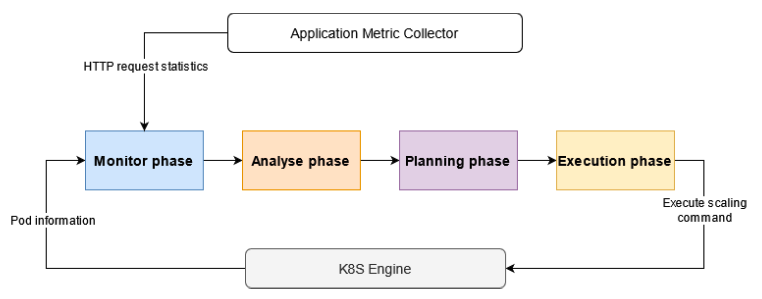
\includegraphics[width=0.8\textwidth]{chapter-2/mape.png}
    \caption{Arsitektur Sistem MAPE, \parencite{riset1}}
    \label{fig:mape}
\end{figure}

\subsection{Penelitian Lainnya}

Adapun \textit{autoscaler} yang sudah dikembangkan dan dibahas di banyak penelitian lain. Pendekatan dan metode yang digunakan sangat variatif. Gambaran umum mengenai penelitian lain yang berhubungan dengan \textit{autoscaler} menggunakan model prediksi, \textit{treshold} atau \textit{rule based} maupun \textit{machine learning} bisa dilihat pada tabel \ref{tab:overview-autoscaler}.

\begin{longtable}{|p{2in}|c|p{1in}|c|p{0.8in}|}

    \caption{Tabel Penelitian Lain terkait Pengembangan Metode \textit{Autoscaling}} \label{tab:overview-autoscaler} \\

    \hline
    \multicolumn{1}{|c|}{\textbf{Paper}} & \textbf{Virtualisasi} & \multicolumn{1}{|c|}{\textbf{Metrik}} & \textbf{Pendekatan} & \multicolumn{1}{|c|}{\textbf{Metode}} \\
    \hline
    \endfirsthead
    %
    \endhead
    %
    \textit{Intelligent Workload Factoring for a Hybrid Cloud Computing Model}, \parencite{zhang} & VM & \textit{Request Rate} & Reaktif & ARIMA \tabularnewline

    \textit{Autonomic Vertical Elasticity of Docker Containers with Elasticdocker}, \parencite{al2017autonomic} & \textit{Container} & Prosesor, Memori & Reaktif & \textit{Rule-based} \tabularnewline

    \textit{Horizontal Pod Autoscaler}, \parencite{hpa2} & \textit{Container} & Prosesor & Reaktif & \textit{Rule-based} \tabularnewline

    \textit{A Novel Resource Prediction and Provisioning Scheme in Cloud Data Center}, \parencite{rpps} & \textit{Container} & Prosesor & Proaktif & ARMA \tabularnewline

    \textit{Workload Prediction Using ARIMA Model and Its Impact on Cloud Applications QoS}, \parencite{workloadprediction} & VM & \textit{Request Rate} & Proaktif & ARIMA \tabularnewline

    \textit{Resource Elasticity Controller for Docker-based Web Applications}, \parencite{resourceelasticity} & \textit{Container} & \textit{Request Rate} & Proaktif & ARIMA \tabularnewline

    \textit{Combining Time Series Prediction Models using Genetic Algorithm to Autoscaling Web Applications Hosted in the Cloud Infrastructure}, \parencite{tspwithga} & - & \textit{Request Rate} & Proaktif & \textit{Genetic Algorithm} \tabularnewline

    \textit{Predicting Cloud Resource Provisioning using Machine Learning Techniques}, \parencite{predictcloudrsrc} & - & \textit{Task Length} & Proaktif & \textit{Artificial Neural Network} \tabularnewline

    \textit{Auto-scaling Microservices on IaaS under SLA with Cost-Effective Framework}, \parencite{asmicrocosteff} & VM & \textit{Request Rate} & Proaktif & \textit{Artificial Neural Network}, \textit{Recurrent Neural Network} \tabularnewline

    \textit{Machine Learning-based Auto-scaling for Containerized Applications}, \parencite{mlbasconapps} & \textit{Container} & \textit{Request Rate} & Proaktif & LSTM \tabularnewline

    \textit{Adaptive Horizontal Scaling of Microservices using Bi-LSTM}, \parencite{adaptivehsmicro} & \textit{Container} & Prosesor, Memori & Gabungan & Bi-LSTM \tabularnewline

    \hline
\end{longtable}
% 
% \section{\textit{Information Retrieval}}
\textit{Information Retrieval} (IR) adalah proses mencari bahan, biasanya berbentuk dokumen, yang bersifat tak terstruktur, biasanya teks, yang memenuhi kebutuhan informasi dari dalam koleksi besar \parencite{introtoinforetri}. IR saat ini sangat sering dilakukan contohnya dalam pencarian informasi berkaitan dengan representasi, penyimpanan, pengaturan, dokumen, halaman web, katalog online, catatan, dan objek multimedia. 

Tujuan utama dari IR adalah penyediaan akses yang efektif dan efisien ke informasi yang dibutuhkan oleh pengguna dalam situasi tertentu. Pengguna IR dapat beragam seperti individu, organisasi, maupun sistem yang membutuhkan informasi yang relevan. IR melibatkan penggunaan teknik-teknik seperti \textit{indexing, searching, retrieval,} dan \textit{evaluation} untuk memastikan informasi yang dihasilkan relevan, tepat, dan sesuai dengan kebutuhan pengguna.

Biasanya IR tersusun oleh beberapa komponen, diantaranya.
\begin{enumerate}
    \item \textit{Indexing}, proses mengubah dokumen menjadi bentuk yang lebih mudah dicari oleh sistem IR.
    \item \textit{Searching}, proses pencarian yang dilakukan oleh pengguna dengan memberikan \textit{query} ke dalam sistem IR dan sistem memberikan keluaran berupa dokumen yang paling relevan.
    \item \textit{Retrieval}, proses sistem IR mengambil dokumen yang relevan dan mengurutkan dokumen berdasarkan kesesuaian dengan \textit{query}.
    \item \textit{Evaluation}, proses penilaian kualitas sistem IR yang biasanya mencakup metrik evaluasi seperti \textit{precision}, \textit{recall}, dan skor F1. 
\end{enumerate}

Dalam melakukan proses-proses tersebut, komponen tersebut menggunakan beberapa teknik, diantaranya.
\begin{enumerate}
    \item \textit{Term Weighting}, teknik pemberian bobot terhadap kata-kata untuk membedakan yang lebih penting dan yang kurang.
    \item \textit{Query Expansion}, teknik menambahkan kata-kata yang relevan pada \textit{query} pengguna untuk meningkatkan akurasi hasil pencarian.
    \item \textit{Clustering}, teknik mengelompokkan dokumen yang mirip untuk memudahkan pengambilan.
\end{enumerate}
% 
% \section{Apache Lucene}
Apache Lucene adalah sebuah perpustakaan atau library open-source untuk Information Retrieval (IR) atau pencarian informasi yang berbasis teks. Lucene adalah \textit{library search engine} yang berkinerja tinggi dan berfitur lengkap. Lucene cocok untuk aplikasi yang memerlukan pencarian terstruktur, pencarian teks lengkap, pencarian pada graf dengan banyak node maupun vektor derajat tinggi, koreksi ejaan, atau saran kueri \parencite{apachelucene}. Lucene dikembangkan di bahasa pemrograman Java dan berfokus pada pencarian teks di dalam dokumen.

Lucene menggunakan model inverted index untuk mempercepat proses pencarian. Model ini mengubah dokumen yang diberikan menjadi indeks kata kunci atau \textit{term} dan menunjukkan letak setiap kata kunci tersebut muncul dalam dokumen. Indeks akan digunakan oleh Lucene untuk mencari kata kunci tertentu dalam dokumen dengan sangat cepat.
% 
% % \section{\textit{Inverted Index}}

\textit{Inverted Index} merupakan struktur data yang biasa digunakan untuk mesin pencari \parencite{invertedindex2}. Tujuan dari implementasi struktur data ini pada mesin pencari adalah untuk mengoptimalkan kecepatan query dalam mencari dokumen yang mengandung kata kunci tertentu. Struktur data ini melakukan pemetaan terhadap kata dan kumpulan tupel yang berisikan \textit{identifier} (ID) dokumen dan posisi karakter \parencite{invertedindex}. Struktur data ini biasanya dipakai untuk menggantikan \textit{Forward Index}. \textit{Forward Index} adalah struktur data yang menyimpan seluruh kata dalam sebuah dokumen sehingga jika \textit{forward index} di-\textit{query}, maka akan memerlukan iterasi sekuensial pada setiap dokumen dan kata kunci untuk membuktikan dokumen relevan. Sumber daya waktu, memori, dan pemrosesan yang dibutuhkan untuk melakukan query semacam itu tidak realistis dan praktis karena nyatanya, mesin pencari harus melakukan hal tersebut ke ratusan hinga jutaan dokumen. Dengan inverted index yang dibuat, query dapat diselesaikan dengan cara langsung melompat ke \textit{identifier} (ID) kata kunci melalui \textit{random access} pada inverted index untuk mendapatkan \textit{identifier} (ID) dokumen dan posisi karakter.
% 
% \section{\textit{Elastic Search}}
% \textit{Elastic Search} adalah aplikasi mesin pencarian RESTful.  \textit{Elastic Search} diciptakan sebagai pembungkus dan inovasi dari Apache Lucene yang sekedar hanya \textit{library} karena aplikasi yang beredar saat ini tidak hanya dibuat di atas Java dan membutuhkan fleksibilitas yang tinggi, sedangkan, Apache Lucene terkenal sangat sulit untuk orang awam yang tidak memahami istilah-istilah dan \textit{information retrieval}. \textit{Elastic Search} sendiri dibuat menggunakan Java namun menggunakan \textit{Application Programming Interface} RESTful melalui protokol HTTP sehingga aplikasi dengan bahasa apapun dapat dengan mudah menggunakan aplikasi ini. Tidak hanya itu, API dari \textit{Elastic Search} ini juga sudah sangat dipermudah sehingga pemakai tidak perlu mengetahui istilah-istilah dalam Apache Lucene. Sehingga, \textit{Elastic Search} ini sangat dekat dengan proses umum pada data seperti menyimpan, membaharui, menghapus, pengindeksan, pencarian, dan sebagainya.

\textit{Elastic Search} merupakan sebuah perangkat lunak \textit{open-source} yang ditulis menggunakan bahasa pemrograman Java. \textit{Elastic Search} dibangun di atas Apache Lucene. \textit{Elastic Search} menyimpan data secara terpusat untuk pencarian secepat kilat dan relevan \parencite{elasticsearchorigin}. Selain Apache Lucene, \textit{Elastic Search} memanfaatkan teknologi-teknologi lain untuk meningkatkan fungsionalitas dan performa, seperti Apache Hadoop untuk big data processing, Apache Spark untuk data analytics, dan Apache Storm untuk real-time stream processing.

\textit{Elastic Search} didesain sebagai sebuah sistem terdistribusi, yang berarti data yang disimpan pada \textit{Elastic Search} akan didistribusikan ke beberapa \textit{node} atau lebih dikenal sebagai \textit{sharding}, sehingga memungkinkan untuk meningkatkan performa, skalabilitas, dan ketahanan pada sistem. Sistem terdistribusi pada \textit{Elastic Search} dapat diatur dan dikonfigurasi agar dapat dijalankan pada beberapa \textit{node} yang terpisah atau pada \textit{cluster} yang terhubung, yang memungkinkan pengguna untuk menyimpan data yang sangat besar dan menjalankan query secara paralel pada beberapa node pada waktu yang bersamaan.

\textit{Elastic Search} dibuat untuk memudahkan pengguna mengakses data dan melakukan pencarian pada data yang besar dan kompleks dengan cepat dan efisien. Meskipun Apache Lucene telah menyediakan fitur-fitur yang bagus untuk \textit{indexing} dan \textit{searching}, tetapi Apache Lucene lebih fokus pada teknologi inti dan pengembangan secara \textit{information retrieval} seperti mengoptimisasi dan pengembangan \textit{indexing} dan \textit{searching}. Hal tersebut menyebabkan penggunaan Lucene memerlukan banyak pengaturan dan konfigurasi tambahan untuk bisa diintegrasikan dengan aplikasi yang lebih besar. Dalam hal ini, \textit{Elastic Search} hadir sebagai sebuah solusi yang lebih terintegrasi, mudah digunakan, dan dapat diatur secara fleksibel. \textit{Elastic Search} memanfaatkan Lucene sebagai mesin pencari, tetapi menambahkan banyak fitur-fitur dan fungsionalitas tambahan untuk meningkatkan performa dan kemudahan penggunaan. Selain itu, \textit{Elastic Search} dirancang sebagai aplikasi dengan sistem terdistribusi dan \textit{scalable} yang memungkinkan data terdistribusi di beberapa node atau \textit{sharding}, sehingga memungkinkan \textit{Elastic Search} untuk mengatasi masalah data yang sangat besar dan kompleks secara efektif dan efisien. Sedangkan, Lucene hanya pada batas kakas atau \textit{library}.

\textit{Elastic Search} dapat digunakan dengan protokol HTTP dan REST API. Dalam penggunaan dengan protokol HTTP, \textit{Elastic Search} menyediakan endpoint API RESTful HTTP yang dapat diakses oleh pengguna dengan memakai klien HTTP, seperti perintah cURL, \textit{Postman} atau \textit{web browser}. Pengguna dapat membuat permintaan HTTP seperti GET, POST, PUT, DELETE ke API endpoint melalui klien HTTP, dan \textit{Elastic Search} akan memberikan respon sesuai dengan permintaan.

Dalam \textit{Elastic Search} terdapat beberapa operasi yang dapat dilakukan, diantaranya:
\begin{enumerate}
    \item \textit{Index}
    
    Operasi ini akan dijelaskan secara khusus pada bagian selanjutnya, \ref{sec:index}.

    \item \textit{Get}
    
    Operasi \textit{Get} digunakan untuk mengambil dokumen individual berdasarkan ID-nya dari indeks tertentu.
    
    \item \textit{Query}
    
    \textit{Query} digunakan untuk melakukan pencarian dan pengambilan data yang sesuai dengan kriteria tertentu. \textit{Elasticsearch} menyediakan berbagai jenis query seperti pencarian teks lengkap, pencocokan kata kunci, pencocokan frasa, pencarian fuzzy, dan lain-lain.
    
    \item \textit{Fetch}
    
    \textit{Fetch} adalah proses pengambilan dokumen lengkap dari indeks setelah melakukan query. Saat ditemukan, \textit{Elasticsearch} mengambil dokumen dari indeks dan akan digunakan sebagai respon kepada pengguna.
    
    \item \textit{Scroll}
    
    \textit{Scroll} adalah mekanisme pengambilan dokumen yang banyak dari hasil pencarian tanpa perlu mengirimkan \textit{query} ulang. Hal ini menyebabkan pengambilan dokumen dapat menjadi lebih efisien dalam beberapa permintaan, namun, dalam beberapa kasus, bisa menjadi lebih lama untuk mengambil semua dokumen yang relevan.
    
    \item \textit{Suggest}
    
    \textit{Suggest} adalah mekanisme untuk memberikan saran atau \textit{autocompletion} saat pengguna memasukkan kata kunci atau frasa. Biasanya digunakan untuk \textit{autocompletion}, pengoreksi kesalahan pengejaan, dan saran pencarian lainnya.
    
    \item \textit{Bulk}
    
    \textit{Bulk} adalah operasi yang digunakan untuk memasukkan atau memperbarui beberapa dokumen dalam satu permintaan.
    
    \item \textit{Flush}
    
    \textit{Flush} adalah operasi yang digunakan untuk mengosongkan memori \textit{cache} dan menulis data yang tertunda ke disk. Operasi ini memastikan bahwa data yang ditulis telah disimpan secara permanen di indeks.
    
    \item \textit{Refresh}
    
    \textit{Refresh} adalah operasi yang digunakan untuk membuat perubahan yang terjadi pada indeks secara terlihat dan dapat dicari. Saat melakukan operasi indeks seperti menambahkan atau menghapus dokumen, perubahan tersebut tidak langsung terlihat oleh pencarian hingga dilakukan operasi refresh.
\end{enumerate}
% 
% \section{Java \textit{Virtual Machine}}
\textit{Java Virtual Machine} atau JVM adalah program yang dapat membaca program java yang telah dikompilasi atau biasa dikenal sebagai \textit{java bytecode} dan menginterpretasikannya menjadi bahasa mesin yang dapat dieksekusi oleh komputer \parencite{java12}. Secara tidak langsung, JVM merupakan komponen utama dalam menjalankan program bahasa Java. Struktur JVM terdiri dari \textit{runtime data structure} di memori dan dua subsistem yang berhubungan langsung dengan \textit{runtime data structure} yaitu \textit{class loader} dan \textit{execution engine}. Semua program yang dibuat dengan Java akan dikompilasi ke \textit{java bytecode} yang nantinya akan diinterpretasikan oleh JVM untuk dieksekusi komputer.

\textit{Elastic Search}, yang terbuat dari bahasa Java, berjalan di atas platform Java Virtual Machine (JVM). JVM sendiri akan bertanggung jawab untuk menjalankan kode Java dan mengelola sumber daya yang dibutuhkan oleh program, seperti memori, prosesor, dan jaringan. Sehingga, JVM memiliki peran penting dalam menjalankan \textit{Elastic Search} dan memastikan performanya baik. JVM menyediakan opsi pengaturan yang membuat pengguna dapat mengontrol alokasi memori dan penggunaan CPU pada aplikasi \textit{Elastic Search}. Dengan mengatur parameter JVM yang tepat, pengguna dapat memperbaiki kinerja \textit{Elastic Search} dan memaksimalkan penggunaan sumber daya sistem.

Parameter yang berhubungan erat dengan alokasi sumber daya pada \textit{Elastic Search} dan mempengaruhi kinerja JVM adalah parameter \textit{heap size} (-Xms dan -Xmx) yang mengatur ukuran \textit{heap memory} yang dialokasikan untuk JVM. \textit{Heap memory} adalah tempat JVM menyimpan objek dan data dari aplikasi Java yang sedang berjalan. Parameter -Xms menentukan ukuran \textit{heap memory} awal yang dialokasikan ketika JVM dimulai, sedangkan parameter -Xmx menentukan batas maksimal ukuran \textit{heap memory} yang dapat dipakai oleh JVM. Selain itu, terdapat parameter lain yang dapat mempengaruhi kinerja JVM dan \textit{Elastic Search}, seperti \textit{thread pool size}, \textit{circuit breaker settings}, dan lain-lain. Parameter-parameter ini dapat diatur melalui file konfigurasi \textit{Elastic Search} atau melalui command line arguments saat menjalankan \textit{Elastic Search}.

% \section{\textit{Indexing}}
\label{sec:index}

\textit{Indexing} adalah suatu teknik untuk menyusun kata-kata dan mengurangi usaha untuk mencari hal yang berkaitan dengan kata tersebut jika diperlukan, \parencite{database}. Secara umum, indeks banyak digunakan pada buku teks, basis data, dan sistem information retrieval. Seperti salah satu contoh tekniknya adalah \textit{Inverted Index} yang telah dijelaskan pada \ref{sec:invertedindex}.

Terdapat kelebihan penggunaan indeks, diantaranya:
\begin{enumerate}
    \item \textit{Indexing} dapat mempercepat proses pencarian data dengan membuat indeks dan mencocokkan kata kunci dengan indeks tersebut, sehingga mesin dapat menemukan data dengan lebih cepat.
    \item \textit{Indexing} dapat meningkatkan akurasi pencarian dengan menampilkan hasil pencarian yang lebih relevan dengan kata kunci yang dimasukkan.
\end{enumerate}

Namun, ada juga kelemahan dari penggunaan indeks, yaitu sebagai berikut.
\begin{enumerate}
    \item \textit{Indexing} memerlukan ruang penyimpanan tambahan untuk membuat indeks.
    \item Proses pembuatan \textit{indexing} memerlukan waktu, terutama jika data yang akan di-indeks sangat banyak.
\end{enumerate}

Sehingga, dapat disimpulkan penggunaan indeks sangat bermanfaat namun menambahkan biaya.
Pada kasus-kasus dokumen besar, penggunaan indeks pengaruhnya sangat besar karena mesin akan mencari data pada indeks terlebih dahulu sebelum mencari data pada dokumen asli. Hal ini dapat membantu mengurangi waktu pencarian dan menghemat penggunaan memori karena mesin tidak perlu membaca seluruh dokumen untuk menemukan data yang dicari. Namun, apabila \textit{indexing} dilakukan secara berlebihan, akan terdapat banyak indeks yang tidak terpakai dan hanya akan menambah kebutuhan memori.

% Konsep \textit{caching} sendiri adalah menyimpan data yang sering diakses pada level cache atau memori yang lebih dekat dengan CPU agar dapat diakses dengan cepat saat ingin melakukan pencarian, lihat gambar \ref{fig:cache-level}. \textit{Cache} sendiri biasanya memiliki ruang yang terbatas sehingga biasanya membuang data yang sudah tidak diakses sehingga jika dibutuhkan harus dicari ke \textit{storage}. Konsep ini ditiru oleh basis data dan aplikasi \textit{information retrieval} untuk mempercepat proses pencarian dengan memanfaatkan \textit{indexing} untuk mencari (lihat gambar \ref{fig:cache-app}) dan \textit{caching} untuk mengembalikan data yang sering diakses dengan memanfaatkan memori.

% \begin{figure}[h]
%     \centering
%     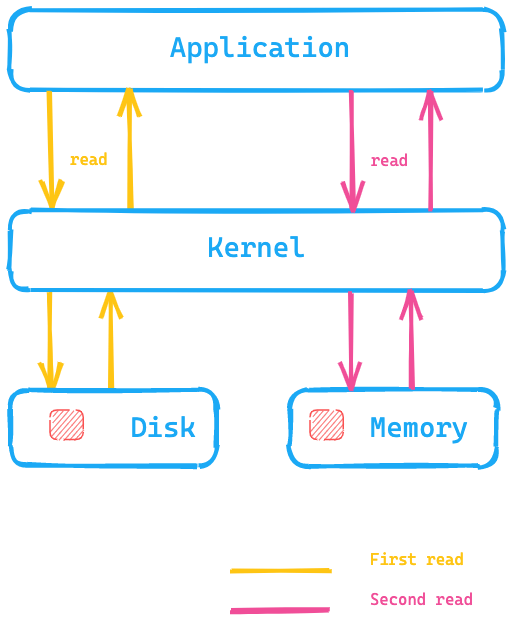
\includegraphics[width=0.5\textwidth]{chapter-2/cache-app.png}
%     \caption{Prinsip Cache pada Aplikasi}
%     \label{fig:cache-app}
% \end{figure}

% \begin{figure}[h]
%     \centering
%     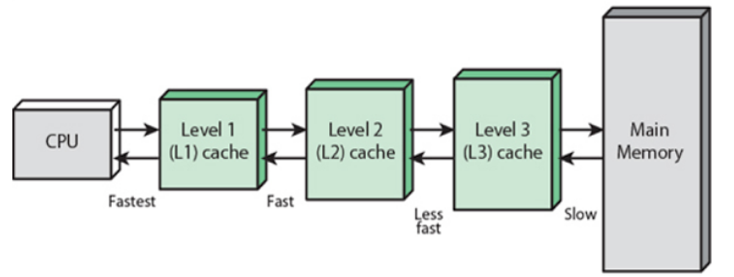
\includegraphics[width=0.5\textwidth]{chapter-2/cache-memory.jpeg}
%     \caption{Level-level pada Cache}
%     \label{fig:cache-level}
% \end{figure}

% \section{\textit{Caching}}

% \section{Simulasi dengan \textit{Elastic Search Benchmarking}}

\textit{Elastic Search Benchmarking} adalah metode yang digunakan untuk melakukan simulasi beban pada \textit{Elastic Search}. Dengan menggunakan \textit{Elastic Search Benchmarking}, pengguna dapat memprediksi jumlah beban yang dapat ditangani oleh \textit{Elastic Search} dan melakukan pencarian terhadap \textit{bottleneck} untuk diperbaiki.

\textit{Elastic Search Benchmarking} memiliki banyak cara pengujian seperti uji beban, uji rentang kisaran, uji keseimbangan, dan uji kestabilan. Uji beban bertujuan untuk mengukur jumlah beban yang dapat ditangani pada suatu waktu tertentu. Uji rentang kisaran dapat digunakan untuk membandingkan kinerja dari setiap rentang data pada variasi yang ada. Uji keseimbangan bertujuan untuk membandingkan kinerja sistem yang memiliki banyak \textit{node} pada sebuah \textit{cluster}. Terakhir, uji kestabilan digunakan untuk menguji kinerja sistem dalam penggunaan waktu yang lama.

\textit{Elastic Search Benchmarking} dapat digunakan untuk memprediksi besar biaya yang diperlukan untuk menjalankan \textit{Elastic Search} pada tingkat beban tertentu. Tak hanya itu, \textit{Elastic Search Benchmarking} dapat digunakan untuk mengidentifikasi titik lemah dan memberikan informasi yang berguna untuk meningkatkan kinerja sistem.

Salah satu tools untuk melakukan \textit{Elastic Search Benchmarking} adalah Rally. Tools ini dapat digunakan untuk mengukur kinerja \textit{Elastic Search} dalam berbagai situasi, termasuk pada lingkungan yang kompleks dan besar. Selain itu, Rally juga menyediakan sejumlah besar skenario pengujian kinerja bawaan yang dapat digunakan untuk menguji kinerja \textit{Elastic Search} dengan berbagai konfigurasi dan skenario pengujian yang berbeda. 
% \section{Pembelajaran Mesin}
% Pembelajaran Mesin adalah sebuah bidang pembelajaran yang mempelajari pemahaman dan membangun metode untuk "belajar" dengan memanfaatkan data untuk meningkatkan banyak aspek terutama efisiensi dan kualitas terhadap suatu rangkaian tugas. Algoritma pembelajaran mesin membangun model berdasarkan data sampel yang biasa disebut \textit{training data} untuk menghasilkan model yang dapat memprediksi atau membuat keputusan tanpa diprogram secara eksplisit, \parencite{ml}.

% \subsection{\textit{Reinforcement Learning}}
% \textit{Reinforcement learning} atau RL adalah bidang pembelajaran mesin yang mengotomasi sebuah agen untuk mengambil tindakan dan memaksimalkan \textit{reward} dari aksi yang dilakukan, \parencite{reinforcementlearning}. RL adalah salah satu paradigma dari tiga pembelajaran mesin dasar seperti \textit{Supervised Learning} dan \textit{Unsupervised Learning}. Singkatnya, RL membuat agen dapat mengoreksi pengetahuannya secara terus menerus agar dapat memaksimalkan fungsinya. Berbeda dengan \textit{Supervised Learning}, RL tidak memerlukan label dan tidak memerlukan secara eksplisit dikoreksi. Fokus dalam membangun RL, adalah mencari keseimbangan eksplorasi terhadap lingkungan baru dan eksploitasi terhadap pengetahuan yang dimiliki.

% penelitian terkait
